\documentclass{article}
\usepackage{hyperref}
\usepackage{listings}
\usepackage{color}
\usepackage{xcolor}
\usepackage{geometry}
\usepackage{graphicx}
\usepackage{amsmath}
\usepackage{caption}
\usepackage{subcaption}
\usepackage[capitalise]{cleveref}
\usepackage{wrapfig}
\usepackage{amssymb}

\geometry{margin=1in}
\pdfminorversion=6

\newcommand\TODO[1]{\textcolor{red}{TODO: #1}}

\newcommand\header[2]{
    \begin{center}
        {\large
        UCSD CSE 167 Assignment #1: \\
        \vspace{0.3cm}
        \Large
        #2}
    \end{center}
}

\definecolor{dkgreen}{rgb}{0,0.6,0}
\definecolor{gray}{rgb}{0.5,0.5,0.5}
\definecolor{mauve}{rgb}{0.58,0,0.82}
\lstset{frame=tb,
        aboveskip=3mm,
        belowskip=3mm,
        showstringspaces=false,
        columns=flexible,
        basicstyle={\small\ttfamily},
        numbers=none,
        numberstyle=\tiny\color{gray},
        keywordstyle=\color{blue},
        commentstyle=\color{dkgreen},
        stringstyle=\color{mauve},
        breaklines=true,
        breakatwhitespace=true,
        tabsize=2
}

% Taken from https://tex.stackexchange.com/questions/83085/how-to-improve-listings-display-of-json-files

\colorlet{punct}{red!60!black}
\definecolor{delim}{RGB}{20,105,176}
\colorlet{numb}{magenta!60!black}

\lstdefinelanguage{json}{
    basicstyle=\normalfont\ttfamily,
    numberstyle=\scriptsize,
    stepnumber=1,
    numbersep=8pt,
    showstringspaces=false,
    breaklines=true,
    frame=lines,
    tabsize=2,
    literate=
     *{0}{{{\color{numb}0}}}{1}
      {1}{{{\color{numb}1}}}{1}
      {2}{{{\color{numb}2}}}{1}
      {3}{{{\color{numb}3}}}{1}
      {4}{{{\color{numb}4}}}{1}
      {5}{{{\color{numb}5}}}{1}
      {6}{{{\color{numb}6}}}{1}
      {7}{{{\color{numb}7}}}{1}
      {8}{{{\color{numb}8}}}{1}
      {9}{{{\color{numb}9}}}{1}
      {:}{{{\color{punct}{:}}}}{1}
      {,}{{{\color{punct}{,}}}}{1}
      {\{}{{{\color{delim}{\{}}}}{1}
      {\}}{{{\color{delim}{\}}}}}{1}
      {[}{{{\color{delim}{[}}}}{1}
      {]}{{{\color{delim}{]}}}}{1},
}

\hypersetup{colorlinks=true}


\begin{document}

\header{3}{3D OpenGL Rendering}

\begin{figure}[ht]
    \centering
    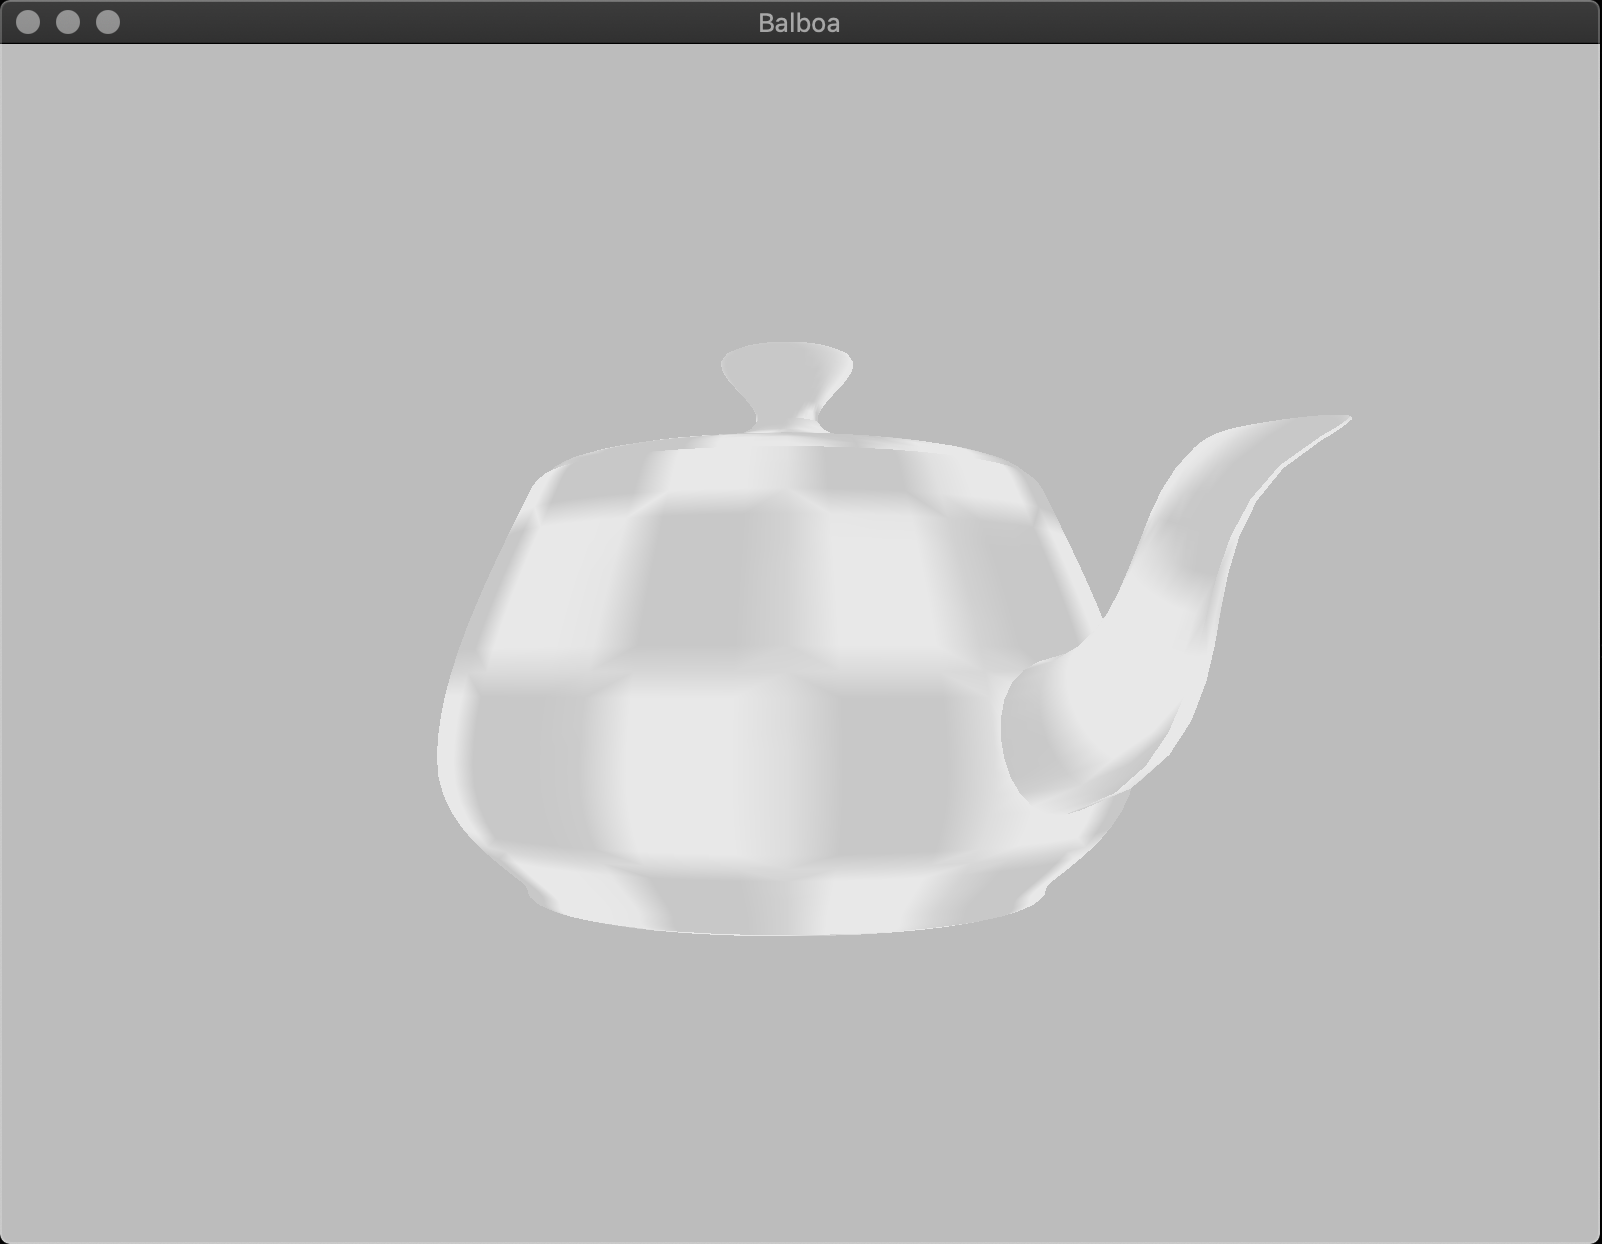
\includegraphics[width=0.40\linewidth]{imgs/hw_3_3_teapot.png}
    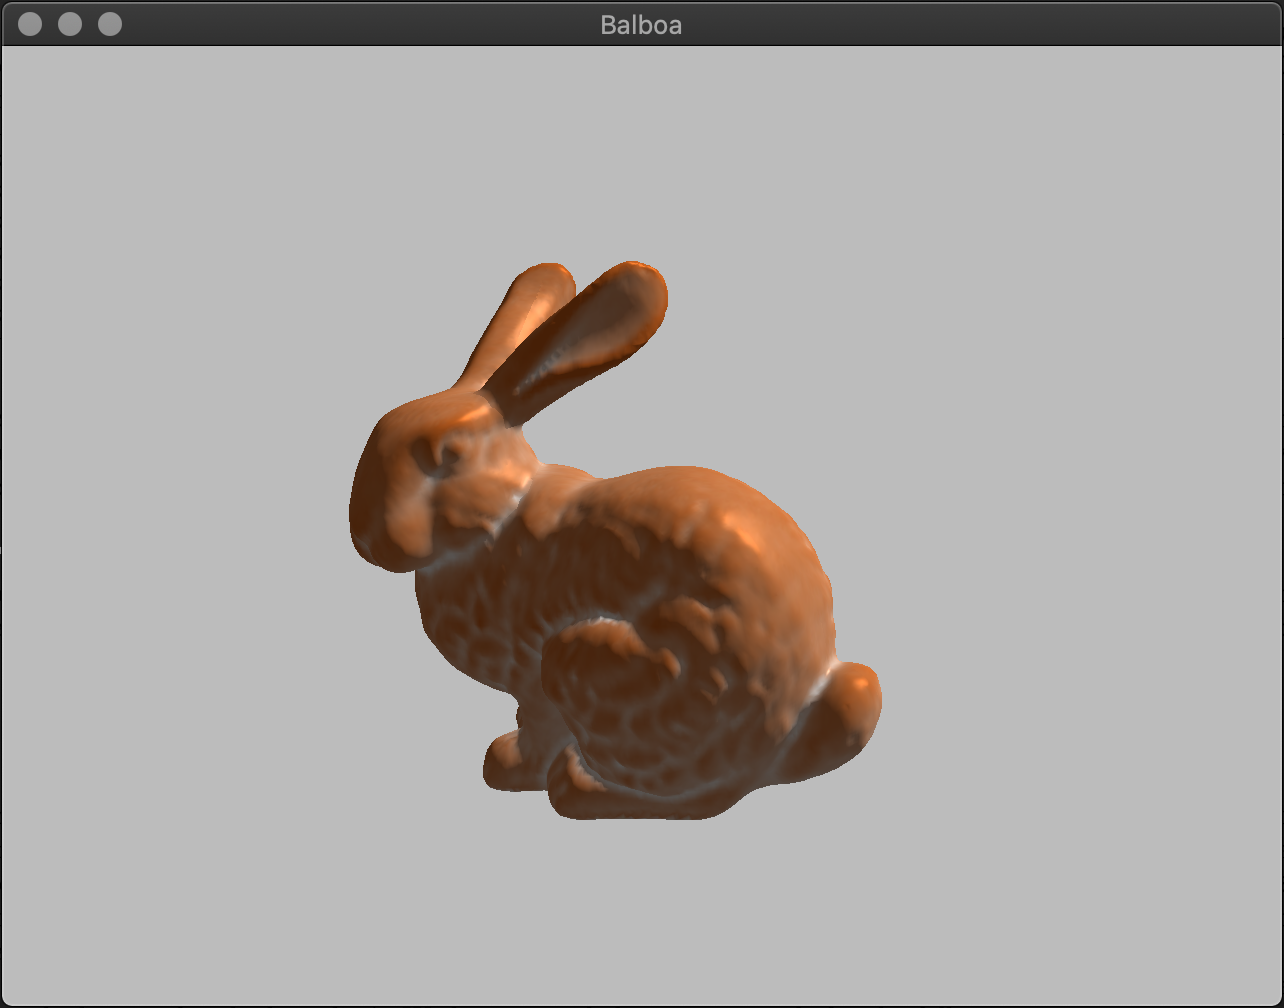
\includegraphics[width=0.40\linewidth]{imgs/hw_3_4_bunny.png}
    \caption{We will develop an interactive interface for inspecting 3D models in this homework.}
    \label{fig:teaser}
\end{figure}

As you can probably tell from the previous homeworks, rendering requires computing interactions between millions of pixels and billions of triangles. This leads to significant challenges in performance, especially when we want to interact with the content in real-time. To make things really fast, pioneers in computer graphics came up with the solution to use \emph{domain-specific hardware} to speedup rendering. Instead of using a general purpose computer to compute everything, we build chips that specialize at rendering. These processors are called the Graphics Processing Units (GPUs). The idea of GPUs can be traced back to more than 40 years ago: The first GPU, \href{https://www.computer.org/publications/tech-news/chasing-pixels/geometry-engine}{Geometry Engine} was developed by Jim Clark and Marc Hannah in 1981. Jim Clark formed the company Silicon Graphics Inc (SGI) in the same year and SGI was one of the most important computer graphics companies in the history. Nowadays, GPUs are found to be general enough to compute very wide-range of computation, including deep learning and many scientific computing tasks, and they are indispensable to the human society. GPU is one of the most successful examples of domain-specific hardware.

In this homework, we will write code to render things using GPUs on your computer. To command your GPUs, we need to send commands to it using some sort of ``Application Programming Interface'' (API). These interfaces are collectively decided by the GPU companies and some other organizations, and each hardware will come with some ``drivers'' that actually implement these interfaces using underlying hardware instructions. The most popular APIs are: \href{https://en.wikipedia.org/wiki/OpenGL}{OpenGL}, \href{https://en.wikipedia.org/wiki/DirectX}{DirectX}, \href{https://en.wikipedia.org/wiki/Metal_(API)}{Metal}, \href{https://en.wikipedia.org/wiki/Vulkan}{Vulkan}, and \href{https://en.wikipedia.org/wiki/WebGPU}{WebGPU}. Among these, DirectX is Windows only, Metal is MacOS only, WebGPU is only for browsers, and Vulkan is extremely low-level and very verbose for providing fine-grained control (it takes literally a thousand lines to render a single triangle in Vulkan). Therefore, we will use OpenGL in this homework: even though DirectX, Metal, and Vulkan are more update to date (the lastest version of OpenGL is 6 years ago), OpenGL is still use in practice and supported by all major GPUs and OSes, and it is significantly easier to learn compared to other lower-level APIs. Just like programming languages, it'll be a lot easier to learn other APIs once you've learned OpenGL.

In this homework, we will mostly follow an online tutorial: \href{https://learnopengl.com/}{learnopengl.com}, because they likely write significantly better tutorials than me. We will implement what we did in the previous homework in OpenGL and hopefully see significant speedup. We will also create a Graphics User Interface (GUI) and enable real-time interaction.

This homework is also more ``open-ended'' compared to the previous ones. We do not ask you to produce the exact same output as we do. At this point, you should be familiar with the theory of rasterization. We're just wrangling with hardware interface, so allowing a bit of creativity seems reasonable.

\section{Creating a window (10 pts)}

Our first task, instead of rendering a single triangle, is to create a window! Read the chapters of \href{https://learnopengl.com/Getting-started/OpenGL}{OpenGL}, \href{https://learnopengl.com/Getting-started/Creating-a-window}{Creating a window}, and \href{https://learnopengl.com/Getting-started/Hello-Window}{Hello Window} in learnopengl.com to see how to create a window with OpenGL context using GLFW. Pick your favoriate background color. We have included GLFW and glad in balboa, so you shouldn't have to download them. We're using OpenGL 3.3, but feel free to use the version you like.

Implement your code in \lstinline{hw_3_1} in \lstinline{hw3.cpp}. Test it using
\begin{lstlisting}[language=bash]
./balboa -hw 3_1
\end{lstlisting}

Once you are done, take a screenshot of the window you created and save it as \lstinline{outputs/hw_3_1.png}.

\section{Rendering a single 2D triangle (20 pts)}

Yeah, it's that time again! Read the \href{https://learnopengl.com/Getting-started/Hello-Triangle}{Hello Triangle} chapter and render a single triangle with constant color (pick one that you like the most). Make sure you've become familiar with the ideas of shaders, VAO, VBO, and EBO. Just to make things slightly different so that we are not just copy and pasting code, let the triangle rotate in the image plane over time (it can be clockwise or counterclockwise, your choice). For the rotation, you can do it whichever way you want, but I recommend you do it in the vertex shader. Read the \href{https://learnopengl.com/Getting-started/Shaders}{Shaders} chapter and understand how to pass in a \lstinline{uniform} variable, then you can use the uniform variable as the rotation angle.  

\paragraph{float vs. double} By default, balboa uses double precision floats through the \lstinline{Real} type. However, by default, GLSL uses single precision floats. Be careful of this discrepancy. You can use \lstinline{Vector3f}/\lstinline{Matrix3x3f} to switch to float in balboa. Also feel free to use the \href{https://github.com/g-truc/glm}{glm} library which is used in the tutorial.

Implement your code in \lstinline{hw_3_2} in \lstinline{hw3.cpp}. Test it using
\begin{lstlisting}[language=bash]
./balboa -hw 3_2
\end{lstlisting}

This time, do a screen recording of your rotating triangle and save it as \lstinline{outputs/hw_3_2.mp4} (or whatever encoding you are using).

\section{Rendering 3D triangle meshes with transformations (35 pts)}

Next, we'll use OpenGL to render the type of scenes we handled in the previous homework. Read the chapters \href{https://learnopengl.com/Getting-started/Transformations}{Transformations}, \href{https://learnopengl.com/Getting-started/Coordinate-Systems}{Coordinate systems}, and \href{https://learnopengl.com/Getting-started/Camera}{cameras}, and that should give you enough knowledge to render the JSON scenes like the ones in the previous homeworks. 

This part is a big jump from the previous parts. I would recommend you to do things incrementally. E.g., handle two 2D triangles first, add projection matrix, add view matrix, add model matrix, handle multiple triangle meshes, and finally add camera interaction.

Below are some notes and tips:

\paragraph{Clip space.} In Homework 2, our projection matrix convert from camera space directly to the screen space. In OpenGL, the hardware expects the projection to convert from camera space to the \emph{clip space}, which by default ranges from $-1$ to $1$ for $x$, $y$, and $z$ axes. Everything outside of the clip space is clipped. Note that the clipping happens at the far side of $z$ as well -- we use the \lstinline{z_far} parameter in the camera in our JSON scene to specify this. The difference in spaces means that we need to use a different projection matrix:
\begin{equation}
\begin{bmatrix}
\frac{1}{as} & 0 & 0 & 0 \\
0 & \frac{1}{s} & 0 & 0 \\
0 & 0 & -\frac{z_{\text{far}}}{z_{\text{far}} - z_{\text{near}}} & -\frac{z_{\text{far}} z_{\text{near}}}{z_{\text{far}} - z_{\text{near}}} \\
0 & 0 & -1 & 0
\end{bmatrix},
\end{equation} 
where $s$ is the scaling/film size parameter as before, and $a$ is the aspect ratio. The first row and the second row scale the $x$ and $y$ clipping plane to $[-1, 1]$ respectively. The third row compresses $z$ values from $-z_{\text{near}}$ to $-z_{\text{far}}$ to $[-1, 1]$. The fourth row is the perspective projection using homogeneous coordinates.

\paragraph{Depth test.} By default, OpenGL does not reject triangles when they are occluded. Remember to turn on depth testing using \lstinline{glEnable(GL_DEPTH_TEST)} and clear the Z buffer (e.g., \lstinline{glClear(GL_COLOR_BUFFER_BIT | GL_DEPTH_BUFFER_BIT)}).

\paragraph{Vertex colors.} In contrast to the learnopengl tutorial, balboa stores the vertex color in a separate array. Therefore it's likely more convienent to create two VBOs:
\begin{lstlisting}[language=C++]
unsigned int VBO_vertex;
glGenBuffers(1, &VBO_vertex);
glBindBuffer(GL_ARRAY_BUFFER, VBO_vertex);
glBufferData(GL_ARRAY_BUFFER, ...);
glVertexAttribPointer(0 /* layout index */,
                      3, GL_FLOAT, GL_FALSE, 3 * sizeof(float), (void*)0);
glEnableVertexAttribArray(0);
unsigned int VBO_color;
glGenBuffers(1, &VBO_color);
glBindBuffer(GL_ARRAY_BUFFER, VBO_color);
glBufferData(GL_ARRAY_BUFFER, ...);
glVertexAttribPointer(1 /* layout index */,
                      3, GL_FLOAT, GL_FALSE, 3 * sizeof(float), (void*)0);
\end{lstlisting}
You only need one VAO per mesh regardless.

\paragraph{Multiple meshes.} To handle multiple meshes in a scene, create a VAO for each mesh.

\paragraph{Window resizing.} We don't require you to handle window resizing in this homework. It's annoying because you'll need to regenerate the projection matrix every time the aspect ratio changes.

\paragraph{Gamma correction.} When we save the image in balboa, we perform a gamma correction by taking a power of $\frac{1}{2.2}$. OpenGL does not by default do this. To enable gamma correction, use \lstinline{glEnable(GL_FRAMEBUFFER_SRGB)}. Read the \href{https://learnopengl.com/Advanced-Lighting/Gamma-Correction}{gamma correction} chapter in learnopengl.com to learn more.

\paragraph{Camera interaction.} Like the tutorial, you should also implement a simple camera interaction scheme, see the \href{https://learnopengl.com/Getting-started/Camera}{Camera} chapter. A simple WSAD style translation suffices. To obtain the camera direction and right vector, you can look at the columns of the \lstinline{cam_to_world} matrix.

As a \textbf{bonus} (15 pts), add camera rotation based on mouse input like the tutorial. Note that the rotation in the tutorial assumes a particular camera frame and would not work for our case. I recommend doing the following: 1) store \lstinline{yaw} and \lstinline{pitch} angles and the original \lstinline{cam_to_world} matrix from the scene. 2) update the \lstinline{yaw} and \lstinline{pitch} based on the mouse movement offsets like in the tutorial. 3) form a rotation matrix \lstinline{R} based on \lstinline{yaw} and \lstinline{pitch}, then form a new \lstinline{cam_to_world} matrix by multiplying the original \lstinline{cam_to_world} matrix with \lstinline{R}. (Don't overwrite the original \lstinline{cam_to_world} matrix!) 

For rotation, it might be tempting to keep only one \lstinline{cam_to_world} matrix by keep multiplying it with new rotation matrices. However, this is going to produce unintuitive behavior (try it!) since yaw and pitch rotations are not \emph{commutative}: applying yaw first then pitch will produce different result compared to applying pitch first then yaw. As a result, when you chain together many pitches and yaws matrix rotations, they will not represent the desired rotation. Yes, rotation is weird. This is why you should explicitly store the \lstinline{yaw} and \lstinline{pitch} angles and modify those instead.

\paragraph{Passing parameters in callback functions.} If you dislike global variables as much as me, you would like the functions \lstinline{glfwSetWindowUserPointer} and \lstinline{glfwGetWindowUserPointer}. You will use it like this:
\begin{lstlisting}[language=C++]
void mouse_callback(GLFWwindow* window, double xpos, double ypos) {
    StructIWanttoPasstoCallback *data_ptr =
        glfwGetWindowUserPointer(window);
}

GLFWwindow* window = glfwCreateWindow(width, height, "Balboa", NULL, NULL);
StructIWanttoPasstoCallback data = ...;
glfwSetWindowUserPointer(window, &data);
glfwSetCursorPosCallback(window, mouse_callback);
\end{lstlisting}

\paragraph{Debugging.} Debugging OpenGL (and other graphics API) programs is painful: if you do one thing wrong, you'll likely get a black screen. The learnopengl tutorial provides \href{https://learnopengl.com/In-Practice/Debugging}{useful tips} for debugging. To debug shaders, it's particularly useful to use a debugger such as \href{https://renderdoc.org/}{renderdoc}. Unfortunately, none of the existing OpenGL debuggers work on MacOS anymore (Apple makes it extremely hard to develop OpenGL on MacOS because they want people to use Metal). For MacOS users, a potential debugging strategy is to emulate the shader on CPU: write the same code on CPU and print out the values, and see if it does what you expect. It's going to be painful regardless, I'm sorry. On the other hand, this is a fruitful research area that awaits innovation to make things better!

For the 3D transformation, copy your Homework 2 code to the \lstinline{parse_transformation} function in \lstinline{hw3_scenes.cpp}. Implement the rest in \lstinline{hw_3_3} in \lstinline{hw3.cpp}.

Test your OpenGL rendering using the following commands:
\begin{lstlisting}[language=bash]
./balboa -hw 3_3 ../scenes/hw3/two_shapes.json
./balboa -hw 3_3 ../scenes/hw3/cube.json
./balboa -hw 3_3 ../scenes/hw3/spheres.json
./balboa -hw 3_3 ../scenes/hw3/teapot.json
./balboa -hw 3_3 ../scenes/hw3/bunny.json
./balboa -hw 3_3 ../scenes/hw3/buddha.json
\end{lstlisting}

For \lstinline{two_shapes} and \lstinline{cube}, they should render to the same images as the previous homework (before you move the camera yourself). The rest are new scenes. (\lstinline{teapot.json} is a higher-resolution version that has 10 times more triangles!) Record a video of you moving the camera for each scene and save them as:
\begin{lstlisting}[language=bash]
outputs/hw_3_3_two_shapes.mp4
outputs/hw_3_3_cube.mp4
outputs/hw_3_3_spheres.mp4
outputs/hw_3_3_teapot.mp4
outputs/hw_3_3_bunny.mp4
outputs/hw_3_3_buddha.mp4
\end{lstlisting}

\paragraph{Acknowledgement.} The bunny model was scanned by Greg Turk and Marc Levoy back in 1994 at Stanford, so it is sometimes called the \href{https://en.wikipedia.org/wiki/Stanford_bunny}{Stanford bunny}. The texture of the bunny model was made by \lstinline{KickAir_8p} who posted the scene in \href{https://blenderartists.org/t/uv-unwrapped-stanford-bunny-happy-spring-equinox/1101297}{blenderarists.org}. The buddha texture was generated by Kun Zhou et al. for their \href{http://kunzhou.net/tex-models.htm}{Texturemontage} paper.

\paragraph{Bonus: textures (15 pts).} Read the \href{https://learnopengl.com/Getting-started/Textures}{Textures} chapter of learnopengl.com and implement textures for the shapes above. We have provided the UV maps for the models except \lstinline{two_shapes} and \lstinline{cube}. I have also included the original textures I used to produce the vertex colors for teapot, bunny, and buddha.

\section{Lighting (25 pts)}
For this part, read the chapters of \href{https://learnopengl.com/Lighting/Colors}{Colors} and \href{https://learnopengl.com/Lighting/Basic-Lighting}{Basic Lighting} in the tutorial, and implement some basic lighting in our viewer. Be careful about the transformation of the normals! Use the vertex colors or texture colors as the \lstinline{objectColor} equivalent in the tutorial. Let's assume \lstinline{ambientStrength=0.1}, \lstinline{specularStrength=0.5} and \lstinline{lightDir} is at \lstinline{normalize(vec3(1, 1, 1))}. 
Note that you can extract the camera position by looking at the fourth column of \lstinline{cam_to_world}.
Also note that the tutorial claimed that it is adding a point light. It is actually a fake point light since it does not have a distance squared falloff. I decided to simplify that part and just use a parallel directional light anyway, which means there is no \lstinline{lightPos} in our case.

The way the tutorial does the lighting requires defining vertex normals (an alternative is to use face normals, but it often looks uglier). We have provided vertex normals for the following scenes:
\begin{lstlisting}[language=bash]
./balboa -hw 3_4 ../scenes/hw3/spheres.json
./balboa -hw 3_4 ../scenes/hw3/teapot.json
./balboa -hw 3_4 ../scenes/hw3/bunny.json
./balboa -hw 3_4 ../scenes/hw3/buddha.json
\end{lstlisting}

Save your output as screenshots:
\begin{lstlisting}[language=bash]
outputs/hw_3_4_spheres.png
outputs/hw_3_4_teapot.png
outputs/hw_3_4_bunny.png
outputs/hw_3_4_buddha.png
\end{lstlisting}

\paragraph{Bonus: lighting animation (10 pts).} Add some animation to the light. Make it move the way you like, and submit a video recording of the animation.

\paragraph{Bonus: different types of lights (10 pts).} Our light currently is a directional light. Implement point lights and spot lights (see the \href{https://learnopengl.com/Lighting/Light-casters}{Light casters} chapter) in your renderer, and support \href{https://learnopengl.com/Lighting/Multiple-lights}{multiple lights}.

\paragraph{Bonus: shadow mapping (20 pts).} Implement a basic shadow map. See the \href{https://learnopengl.com/Advanced-Lighting/Shadows/Shadow-Mapping}{Shadow Mapping} chapter in learnopengl. Support of directional lights is good enough. 

\section{Design your own scenes (10 pts)}
We're at the fun part again. Design your own scene and render it using your new renderer!

%\bibliographystyle{plain}
%\bibliography{refs}

\end{document}
